
The directivity of a sound sources is an issue that has an impact on many situations of our daily life, e.g. at live music venues. Voluntary listeners, namely the audience, enjoy comparatively high sound pressure levels when gathering around the stage. Non-voluntary listeners, generally neighbours, tend to perceive the sound emitted by the stage as a disturbing noise. This problem might be minimized with directivity control of the sound sources. The high sound energy will then be emits towards the audience, and less towards the neighbours. 


There are several effects that make this difficult, because commonly used loudspeaker contraptions for low frequency playback tend to act like omnidirectional sound sources \citep[p. 1391 f.]{crocker98}.  First, the dampening of sound in the air has significantly less influence on sound towards the lower frequency of the human hearing range than it has towards the higher frequency \citep[p. 240]{moeser2009}. Secondly, because of the way most houses are built, low frequency sound penetrates through walls and windows much more than high frequency sound \citep[p. 240 ff.]{moeser2009}. All of these effects lead to neighbours being disturbed by \textit{the low frequency} from nearby live music venues.\\
The difference in the perception of the sound is visualised in \autoref{fig:Problem}.


\begin{figure}[htbp]
	\centering
	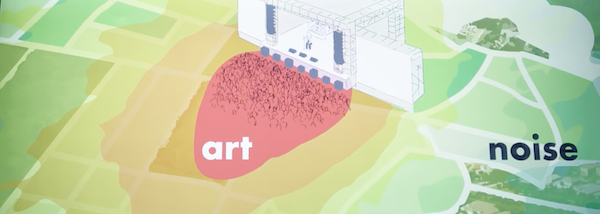
\includegraphics[width=1\textwidth]{change_later.png}
	\caption{Normalized \gls{spl} in colour, red is high \gls{spl} where blue is low \gls{spl}}
		\label{fig:Problem}
\end{figure}

%\autoref{fig:Problem} shows the total sound pressure level \gls{spl} in \gls{db} from \SI{20}{\hertz} to \SI{20}{\kilo\hertz} for the voluntary listeners and the non-voluntary listeners during a concert.
\autoref{fig:Problem} shows a qualitative drawing of a near-ideal sound pressure distribution in the vicinity of a stage during a concert. The high-\gls{spl}areas are highlighted by red color, and is the area where the voluntary listeners condense. This area is define as the \textbf{participants' area} The non-voluntary listeners are located in the area around the participants' area, that we define as \textbf{the neighbourhood}. 

While a \gls{spl} distribution as depicted in \autoref{fig:Problem} is easier to achieve the higher the frequency gets, towards low frequencies the \gls{spl}distribution might look more like depicted in autoref(fig:problem2).



The directivity control of mid- and high frequency has a known solution which has been applied for many years. In general, horns are used, which are designed for a particular radiation pattern. Due to the long wave length in the low/mid- and low frequency range, the horns that are required to direct those wavelengths are not feasible for practical applications due to their size and weight. Therefore other, more space saving solutions have been developed and implemented in the last decade. It is possible to achieve a cardiod emission pattern by arranging subwoofers in a particular manner. Two or three subwoofers are pointed towards the participants' area and one subwoofer is pointed the opposite way \citep{KS28}. The signal for the subwoofer pointing away from the audience is processed to manipulate the phase.


This project aims towards applying a principle that has been put into commercial use in the D\&B audiotechnik SL-series, where the low/mid frequency directivity is controlled by signal processing four speaker unit. Two units are arranged in the front of the line array module and the other two arranged on each of the sides of the line array module.



\section{preliminary problem statement}
The following questions are made with the intention of gathering the necessary knowledge, to be able to answer a later stated problem statement. The preliminary questions, which will be answered in the analysis, are:

\begin{itemize}
\item In which frequency area do the line source speaker behave omnidirectional?
\item Which known technique is used to do the speaker cardioid?
\item Can a simulation be made which support D\&B audiotechnik claim?
\item Does beam forming of a line source speaker benefit in a room environment ?
\end{itemize}



